%----------------------------------------------------------------------------
\chapter{Tesztelési terv}
%----------------------------------------------------------------------------

%----------------------------------------------------------------------------
\section{Időzített automata generátor tesztelése}
%----------------------------------------------------------------------------

A generált időzített automaták forráskodját unit tesztek segítségével szeretnénk tesztelni.
Az Xtext keretrendszer által nyujtott eszközök erre célra jól alkalmazhatok.

\begin{figure}[!ht]
    \centering
    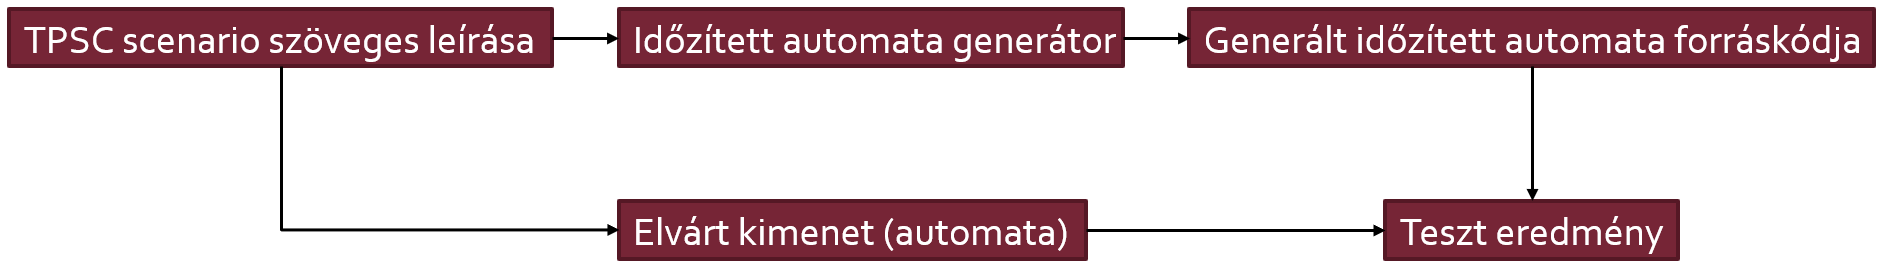
\includegraphics[width=150mm, height=9cm, keepaspectratio]{figures/unit_test_flow.png}
    \caption{Unit tesztelés folyamatábrája.}
\end{figure}

A 9.1. ábrán látható a unit tesztelés tervének folyamatábrája.
A teszteléssel az a célunk, hogy minél nagyobb magabiztosággal biztosítjuk a generátor helyes működését.
Tesztelési kategoriák:

\begin{itemize}
    \item Üzenet típusok egyenkénti tesztelése
    \item Üzenet típusokból összeállított kombinációk tesztelése
    \item Scenario operátorok tesztelése
\end{itemize}

Az üzenet típusok egyenkénti tesztelésénél az összes üzenet típust le szeretnénk fedni.
Az üzenet kombinációkból a főbb eseteket szeretnénk tesztelni.
Például sima üzenet után required üzenet és ezek váltakozása a fail üzeneteket is bele értve.
A scenario operátoroknál azt fontos tesztelni, hogy a különálló üzenetekhez tartozó automata minták jól illeszkedjenek a operátorral elátott üzenetek automatájával.

Egy unit teszt akkor sikeres ha a generált automata forráskódja megegyezik az elvárt automata forráskodjával.

%----------------------------------------------------------------------------
\clearpage\section{Monitor forráskód generátor tesztelése }
%----------------------------------------------------------------------------

A generált monitor forráskodját integrációs tesztek segítségével szeretnénk tesztelni.
Az Xtext keretrendszer a specifikált dsl nyelvhez generál egy maven plugin-t.
Ezt a plugin-t betölthetjük egy egyszerű maven projektbe és használhatjuk is az elkészített dsl nyelvünket.

\begin{figure}[!ht]
    \centering
    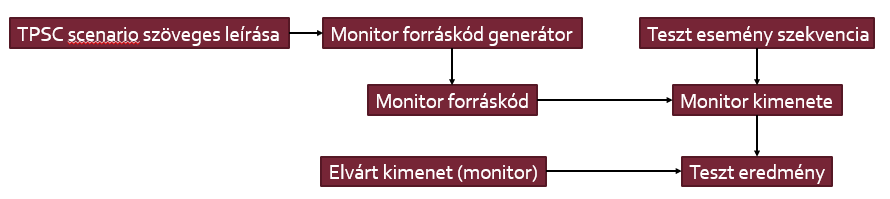
\includegraphics[width=150mm, height=9cm, keepaspectratio]{figures/integration_test_flow.png}
    \caption{Integrációs tesztelés folyamatábrája.}
\end{figure}

A 9.2. ábrán megtekinthető az integrációs tesztelés tervének folyamatábrája.
A következők tesztelési kategoriáink:

\begin{itemize}
    \item Scenario operátorok tesztelése
    \item Üzenet paraméterek tesztelése
    \item Időzítések tesztelése
\end{itemize}

A scenario operátorok tesztelésénél az a célunk, hogy a monitor a követelmény különböző ágait figyelembe véve helyes kimenetet adjon.
Például loop operátor esetén a minimum, köztes és maximum üzenet szekvencia ismétléseknél is helyes legyen a monitor kimenete.
Ha a maximumnál többször szerepel az üzenet szekvencia akkor hibát kell, hogy jelezen.
Üzenet paraméterek tesztelése esetén azt szeretnénk vizsgálni, hogy a monitor helyesen értelmezi e az üzenet paramétereket.
Az időzítések tesztelésénél az a fontos, hogy a monitor képes-e az óraváltozók alapján az időzitési feltételeket kiértékelni.
Például ha az üzenet a feltétel alapján időben érkezik meg akkor helyes kimenetet adjon
, vissza ha feltétel szerint később érkezik meg akkor a monitornak hibát kell jeleznie.

Egy integrációs teszt akkor sikeres ha a monitor kimenete megegyezik az elvárt kimenettel.